\documentclass[11pt,spanish,listoffigures]{tfgetsinf}
\usepackage[utf8]{inputenc} 

%%%%%%%%%%%%%%%%%%%%%%%%%%%%%% PORTADA %%%%%%%%%%%%%%%%%%%%%%%%%%%%%%

\title{Implementación de un API Gateway para una arquitectura de microservicios}
\author{Alejandro Carrión Sanmartín}
\tutor{Patricio Letelier Torres}
\curs{2020-2021}

%%%%%%%%%%%%%%%%%%%%%%%%%%%%%% PALABRAS CLAVE %%%%%%%%%%%%%%%%%%%%%%%%%%%%%%

\keywords{????, ?????????, ????, ?????????????????} % Paraules clau 
         {?????, ???, ???????????????}              % Palabras clave
         {?????, ????? ?????, ?????????????}        % Key words

\begin{document}

%%%%%%%%%%%%%%%%%%%%%%%%%%%%%% RESUMEN %%%%%%%%%%%%%%%%%%%%%%%%%%%%%%

\begin{abstract}
????
\end{abstract}
\begin{abstract}[catalan]
????
\end{abstract}
\begin{abstract}[english]
????
\end{abstract}

\mainmatter

%%%%%%%%%%%%%%%%%%%%%%%%%%%%%% INTRODUCCIÓN %%%%%%%%%%%%%%%%%%%%%%%%%%%%%%

\chapter{Introducción}

Este tfg surge en el contexto de una práctica en empresa.

No habrà tfgs relacionados en la etsinf xk normalmente se usa productos hechos. Se va a creat uno propio xk está relacionado con el sistema de despliegue.

\section{Motivación}

La principal motivación de este proyecto es resolver un problema real. Este consiste en otorgar a una aplicación con arquitectura de microservicios la capacidad de ocultarlos, así como permitir la ejecución simultánea de más de una instancia de los mismos. Cabe destacar que la aplicación en cuestión se encuentra todavía en fase de desarrollo y que el API Gateway que se va a realizar como solución es un punto clave en su arquitectura, como se detallará más adelante.

Primero de todo, una arquitectura orientada a microservicios es aquella formada por servicios independientes, ejecutados en procesos diferentes, que se encargan de realizar funciones concretas y que trabajan de forma conjunta para lograr el objetivo u objetivos globales de la aplicación. Para ilustrar mejor este enfoque arquitectónico, se muestra a continuación un diagrama que representa una aplicación cuyo backend está formado por los microservicios de “Clientes”, “Vendedores” y “Compras”:

\begin{figure}
	\centering
	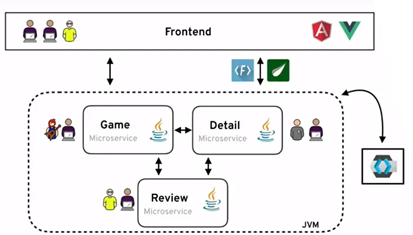
\includegraphics{images/a}
	\caption{Aplicación con arquitectura de microservicios básica}
\end{figure}

La comparativa de esta aproximación frente a la arquitectura tradicional monolítica es la siguiente:

\begin{itemize}

	\item Posibilidad de desplegar en diferentes máquinas
No es necesario disponer de un servidor moderno con mucha capacidad de cómputo, se puede utilizar servidores más pequeños alojados, además, en diferentes lugares. Sin embargo, una aplicación hecha por microservicios puede ser potencialmente desplegada en la misma máquina si se requiere.

	\item Multi instancia
Se puede ejecutar más de una instancia del mismo microservicio de manera simultánea en máquinas diferentes. Esto permite realizar balanceo de carga y hace que no se constituya un punto único de fallada. No obstante, esto puede acarrear otros problemas como puede ser el uso bases de datos diferentes entre instancias del mismo microservicio, lo que supondría tener un mecanismo de unificación y actualización.

	\item Uso de diferentes tecnologías
Cada microservicio puede estar construido con una tecnología diferente y puede utilizar diferentes mecanismos de persistencia tales como bases de datos SQLite, SQL Server o archivos XML. Permite adaptar la tecnología a las necesidades concretas de cada parte de la aplicación, por ejemplo, puede ser interesante desarrollar un microservicio de inteligencia artificial con una tecnología más puntera y enfocada a este ámbito.

	\item Mejor maniobrabilidad en los despliegues
Ante cualquier cambio no es necesario desplegar la aplicación entera, solamente los microservicios implicados en el cambio. Esto reduce los tiempos para volver a poner en marcha el software en cuestión, incluyendo compilación, publicación, distribución y otras tareas que puedan ser necesarias. Por contraparte, no hay que olvidar que este proceso se puede complicar debido a que la aplicación posiblemente esté distribuida en varias máquinas.

	\item Reutilización en diferentes aplicaciones
Ciertos microservicios, como los que se ocupan del sistema de autenticación o de la gestión de los permisos de cada usuario, son necesarios en una gran mayoría de aplicaciones, por lo que pueden ser reutilizados si se construyen con ese fin. Las aplicaciones monolíticas tienen un grado fuerte de acoplamiento y no tienen esta flexibilidad, sin embargo, suelen ser más eficientes al estar hechas por código exclusivo para ellas.

	\item Mejor mantenibilidad
Mantener aplicaciones con este enfoque suele ser más sencillo debido a la separación funcional que va ligada a los microservicios, son componentes independientes. Ahora bien, no hay que olvidar que el hecho de ejecutarse en diferentes procesos y, posiblemente, en diferentes máquinas hace que las comunicaciones entre ellos pueda ser un tema delicado y requiere un trabajo extra.

	\item Escalabilidad
Los microservicios, y la separación de funcionalidad que otorgan, facilitan el escalado de las partes de la aplicación que así lo requieran de una manera más fácil.

	\item Especialización de equipos
Se puede tener personas o equipos centrados en microservicios concretos, lo que facilita el desarrollo y mantenimiento de la aplicación al no obligar a los desarrolladores a cambiar de contexto en exceso entre varios componentes. Por otro lado, si todos los microservicios siguen un mismo patrón arquitectónico, puede ser relativamente sencillo para un desarrollador adaptarse a uno en el que no ha trabajado nunca.

	\item Despliegue continuo
Se adapta muy bien a procesos de integración continua y despliegue continuo, se trata de una práctica que está en auge hoy en día.

\end{itemize}

Se puede obtener más información acerca de los microservicios en el artículo de James Lewis y Martin Fowler titulado “Microservices” [1].
Centrándonos en el tema central del proyecto, un API Gateway, o Gateway para abreviar, se entiende como un componente que se interpone entre la interfaz de usuario (frontend) de una aplicación y los servicios en los que se basa (backend). Actúa como intermediario y es el único punto de entrada al mencionado backend.
Como se aprecia en la definición anterior, un Gateway puede ser implementado tanto en arquitecturas monolíticas como en las de microservicios, si bien constituye una parte fundamental en las segundas. Con él se consigue que estos pequeños servicios no tengan que conocerse entre ellos y que puedan tener varias instancias en ejecución al mismo tiempo. El punto realmente importante es el segundo, pues es una de las ventajas antes comentadas de este enfoque arquitectónico.

\begin{figure}
	\centering
	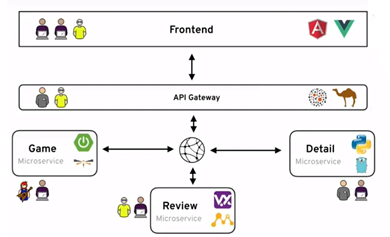
\includegraphics{images/b}
	\caption{Aplicación con arquitectura de microservicios con API Gateway}
\end{figure}

\section{Objetivos}

?????

\section{Estructura del documento}

?????

%%%%%%%%%%%%%%%%%%%%%%%%%%%%%% CONTEXTO TECNOLÓGICO %%%%%%%%%%%%%%%%%%%%%%%%%%%%%%

\chapter{Contexto tecnológico}

•	AWS API Gateway: Situada para manejar todas las interacciones alrededor de las llamadas API, el API Gateway de Amazon maneja las API REST y websocket y funciona muy bien con el resto del ecosistema de AWS.

•	Apigee: Ahora parte del ecosistema de productos para desarrolladores de Google, el gateway Apigee incluye muchas herramientas no solo para administrar las API, sino también para crearlas.

•	Kong: Mencionado anteriormente, Kong es una alternativa de código abierto que ofrece todas las características principales que hemos mencionado en este artículo.

•	Tyk: Otra opción de código abierto, Tyk es una puerta de enlace API popular que ofrece las características principales que esperaría para las API y una arquitectura de microservicios, pero también ofrece un conjunto de herramientas adyacentes que funcionan con sus ofertas de servicios.

•	WSO2, AWS API Gateway, Kong, 42crunch y 3scale


%%%%%%%%%%%%%%%%%%%%%%%%%%%%%% ANÁLISI DEL PROBLEMA %%%%%%%%%%%%%%%%%%%%%%%%%%%%%%

\chapter{Análisis del problema}

?????

\section{Especificación de requisitos}

?????

\section{Soluciones posibles}

?????

\section{Solución propuesta}

?????

\section{Plan de trabajo}

?????

%%%%%%%%%%%%%%%%%%%%%%%%%%%%%% DISEÑO DE LA SOLUCIÓN %%%%%%%%%%%%%%%%%%%%%%%%%%%%%%

\chapter{Diseño de la solución}

?????

\section{Arquitectura del sistema}

?????

\section{Diseño detallado}

?????

\section{Tecnología utilizada}

?????

\section{Metodología software}

?????

\section{Mantenimiento y gestión de versiones}

?????

%%%%%%%%%%%%%%%%%%%%%%%%%%%%%% DESARROLLO DE LA SOLUCIÓN %%%%%%%%%%%%%%%%%%%%%%%%%%%%%%

\chapter{Desarrollo de la solución}

?????

%%%%%%%%%%%%%%%%%%%%%%%%%%%%%% PRUEBAS %%%%%%%%%%%%%%%%%%%%%%%%%%%%%%

\chapter{Pruebas}

?????

%%%%%%%%%%%%%%%%%%%%%%%%%%%%%% CONCLUSIONES %%%%%%%%%%%%%%%%%%%%%%%%%%%%%%

\chapter{Conclusiones}

?????

%%%%%%%%%%%%%%%%%%%%%%%%%%%%%% BIBLIOGRAFÍA %%%%%%%%%%%%%%%%%%%%%%%%%%%%%%

\begin{thebibliography}{10}

\bibitem{WAR}
   J. Lewis y M. Fowler.
   \newblock \textit{Microservices}.
   \newblock Consultado en 
   \url{https://martinfowler.com/articles/microservices.html}.

\end{thebibliography}
\cleardoublepage

\end{document}
